\documentclass{beamer}
\mode<presentation>
\usepackage{amsmath}
\setbeamertemplate{itemize items}[circle] 
\setbeamercolor{itemize item}{fg=black}
\usepackage{amssymb}
%\usepackage{advdate}
\usepackage{adjustbox}
\usepackage{subcaption}
\usepackage{enumitem}
\usepackage{multicol}
\usepackage{mathtools}
\usepackage{listings}
\usepackage{url}
\usepackage{etex}
\def\UrlBreaks{\do\/\do-}
\usetheme{metropolis}
\setbeamertemplate{footline}
{
  \leavevmode%
  \hbox{%
  \begin{beamercolorbox}[wd=\paperwidth,ht=2.25ex,dp=1ex,right]{author in head/foot}%
    \insertframenumber{} / \inserttotalframenumber\hspace*{2ex} 
  \end{beamercolorbox}}%
  \vskip0pt%
}
\setbeamertemplate{navigation symbols}{}

\providecommand{\nCr}[2]{\,^{#1}C_{#2}} % nCr
\providecommand{\nPr}[2]{\,^{#1}P_{#2}} % nPr
\providecommand{\mbf}{\mathbf}
\providecommand{\pr}[1]{\ensuremath{\Pr\left(#1\right)}}
\providecommand{\qfunc}[1]{\ensuremath{Q\left(#1\right)}}
\providecommand{\sbrak}[1]{\ensuremath{{}\left[#1\right]}}
\providecommand{\lsbrak}[1]{\ensuremath{{}\left[#1\right.}}
\providecommand{\rsbrak}[1]{\ensuremath{{}\left.#1\right]}}
\providecommand{\brak}[1]{\ensuremath{\left(#1\right)}}
\providecommand{\lbrak}[1]{\ensuremath{\left(#1\right.}}
\providecommand{\rbrak}[1]{\ensuremath{\left.#1\right)}}
\providecommand{\cbrak}[1]{\ensuremath{\left\{#1\right\}}}
\providecommand{\lcbrak}[1]{\ensuremath{\left\{#1\right.}}
\providecommand{\rcbrak}[1]{\ensuremath{\left.#1\right\}}}
\theoremstyle{remark}
\newtheorem{rem}{Remark}
\newcommand{\sgn}{\mathop{\mathrm{sgn}}}
\providecommand{\abs}[1]{\left\vert#1\right\vert}
\providecommand{\res}[1]{\Res\displaylimits_{#1}} 
\providecommand{\norm}[1]{\lVert#1\rVert}
\providecommand{\mtx}[1]{\mathbf{#1}}
\providecommand{\mean}[1]{E\left[ #1 \right]}
\providecommand{\fourier}{\overset{\mathcal{F}}{ \rightleftharpoons}}
%\providecommand{\hilbert}{\overset{\mathcal{H}}{ \rightleftharpoons}}
\providecommand{\system}{\overset{\mathcal{H}}{ \longleftrightarrow}}
	%\newcommand{\solution}[2]{\textbf{Solution:}{#1}}
%\newcommand{\solution}{\noindent \textbf{Solution: }}
\providecommand{\dec}[2]{\ensuremath{\overset{#1}{\underset{#2}{\gtrless}}}}
\newcommand{\myvec}[1]{\ensuremath{\begin{pmatrix}#1\end{pmatrix}}}
\let\vec\mathbf

\lstset{
%language=C,
frame=single, 
breaklines=true,
columns=fullflexible
}

\numberwithin{equation}{section}

\title{Probability}
\author{Faraz Patnam\\ Dept. of Electrical Engg.,\\IIT Hyderabad.}

\date{\today} 
\begin{document}

\begin{frame}
\titlepage
\end{frame}

\section*{Outline}
\begin{frame}{Table of Contents}
    \tableofcontents
\end{frame}

\section{Problem}
\begin{frame}{Problem Statement}
    The number lock of a suitcase has 4 wheels, each labeled with ten digits i.e., from 0 to 9. The lock opens with a sequence of four digits with no repeats. What is the probability of a person getting the right sequence to open the suitcase?
\end{frame}

\section{Solution}
\subsection{Total Number of outcomes}
\begin{frame}{\textbf{Total Number of Possible Sequences}}
    \begin{itemize}
        \item Each wheel has $10$ possible digits and no digit repeats in the sequence.
        \item To get all the possible values of the sequence we need to arrange all the ten digits (0 to 9) in four places. (No repetitions)
        \item The total number of possible sequences is:
        \begin{align}
            \myvec{10 \\ 4} \times {4!} = 5040
        \end{align}
        \item or 
        \begin{align}
            10 \times 9 \times 8 \times 7 = 5040
        \end{align}
    \end{itemize}
\end{frame}

\begin{frame}{\textbf{Total Number of Possible Sequences}}
    This is because 
    \begin{itemize}
        \item The first wheel has 10 possible digits.
        \item The second wheel has nine possible digits (since one digit has already been used).
        \item The third wheel has 8 possible digits.
        \item The fourth wheel has 7 possible digits.
    \end{itemize}
\end{frame}

\subsection{Probability of Success}
\begin{frame}{\textbf{Probability of Success}}
    Out of all 5040 possibilities, only onesequence is right. The probability $p$ of guessing the right sequence 
    \begin{align}
        p &= \frac{1}{\text{Total number of possible sequences}}\\ &= \frac{1}{5040}\\ &= 0.000198
    \end{align}
\end{frame}

\subsection{Random Variable}
\begin{frame}{Defining the Random Variable}
    We model this problem using Bernoulli random variables,\\
    Let $X$ be the random variable that represents the correct sequence of digits of the Wheel:
    \begin{itemize}
        \item $X = 1$ , If the sequence chosen is correct,
        \begin{align}
            \text{\brak{\text{With probability }p = \frac{1}{5040}}}
        \end{align}
        \item $X = 0$, If the sequence chosen is incorrect,
        \begin{align}
            \text{\brak{\text{With probability } 1 -p = \frac{5039}{5040}}}
        \end{align}
    \end{itemize}
\end{frame}

\subsection{PMF}
\begin{frame}{\textbf{Probability Mass Function (PMF)}}
        The PMF  of a Bernoulli random variable $X$ is given by:
    \begin{align}
	P\brak{X = x} = p^x\brak{1 - p}^{1 - x}, x \in \cbrak{0,1}
    \end{align}
    substituting $p = \frac{1}{5040}$,\\
    \begin{align}
     P\brak{X = 1} = 0.000198, P\brak{X = 0} = 0.999802
    \end{align}
    \begin{align}
    	P\brak{X = x} = \begin{cases}
    		0.000198, & x = 1 \\
    		0.999802, & x = 0 \\
    		0, & \text{otherwise}
    	\end{cases}
    \end{align}
\end{frame}

\begin{frame}{PMF Plot}
    \begin{figure}
        \centering
        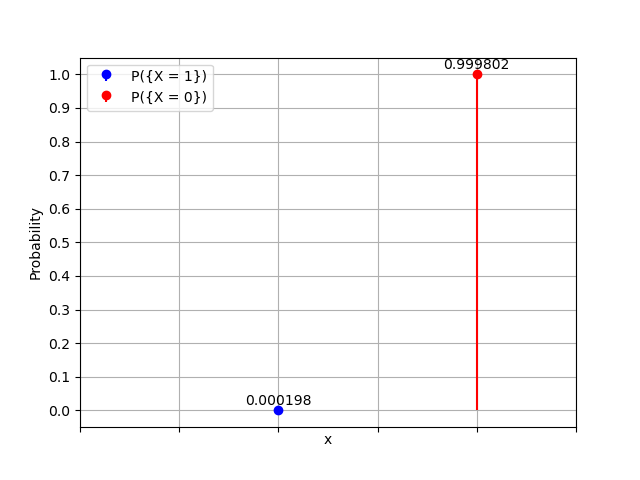
\includegraphics[width=0.8\linewidth]{figs/pmf.png}
        \caption{Probability Mass Function}
        \label{fig:enter-label}
    \end{figure}
\end{frame}

\subsection{CDF}
\begin{frame}{\textbf{Cumulative Distribution function (CDF)}}
    The CDF of a discrete random variable is defined as:\\
    \begin{align}
    	F_X\brak{x} = P\brak{X \leq x}
    \end{align}
    \begin{align}
            F_X\brak{x} = \begin{cases}
                    0, & x < 0 \\
                    0.999802, & 0 \leq x < 1  \\
                    1, & x \geq 1
            \end{cases}
    \end{align}
\end{frame}

\begin{frame}{CDF Plot}
    \begin{figure}
        \centering
        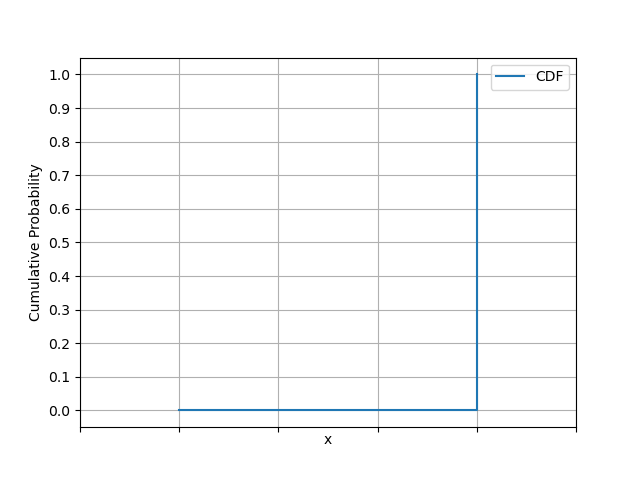
\includegraphics[width=0.8\linewidth]{figs/cdf.png}
        \caption{Cummulative Distribution Function}
        \label{fig:enter-label}
    \end{figure}
\end{frame}
\end{document} 
